% vim: set textwidth=78 autoindent:

\section{Interpolationsplugin}\index{Plugins!Interpolation}

% when the revision of a chapter has been finalized, 
% comment out the following line:
%\updatedisclaimer

Das Plugin \toolbtntwo{interpolation}{Interpolation} erlaubt es, ein TIN
(Triangulated Irregular Network) oder eine IDW (Inverse Distance Weighted)
Interpolation aus Vektorpunkten zu berechnen. Die Anwendung ist sehr einfach
zu bedienen und bietet ein intuitives Interface, wie in
Abbildung~\ref{fig:interpolation_dialog} zu sehen. Die folgenden Parameter
m�ssen angegeben werden, damit das Plugin funktioniert:

\begin{itemize}[label=--]
\item \textbf{Eingabevektor}: W�hlen Sie einen in QGIS geladenen Vektor
Punktlayer. Wenn mehrere Layer angegeben werden, werden die Daten aller Layer
f�r die Interpolation verwendet. Beachten Sie auch, dass es m�glich ist,
Linien und Polygone als Randbedingungen f�r die Triangulation zu verwenden,
indem Sie im Dropdown-Men� ``Typ'' des geladenen Layers entweder
Strukturlinien oder Bruchkanten ausw�hlen.
\item \textbf{Interpolationsattribut}: W�hlen Sie die Attributspalte mit den
Werten f�r die Berechnung oder aktivieren Sie das Kontrollk�stchen
\checkbox{Z-Koordinate f�r Interpolation verwenden}.
\item \textbf{Interpolationsmethode}: W�hlen Sie als Interpolationsmethode
\selectstring{Unregelm��iges Dreiecksnetz (TIN)}{} oder \selectstring{Inverse
Distanzgewichtung (IDW)}{}.
\item \textbf{Spalten- und Zeilenanzahl}: Definieren Sie �ber die Spalten-
und Zeilenanzahl die Aufl�sung der Ausgabekarte.
\item \textbf{Ausgabedatei}: Legen Sie einen Namen f�r den Ausgabelayer fest.
\end{itemize}

\begin{figure}[ht]
   \begin{center}
   \caption{Dialog Interpolationsplugin \nixcaption}\label{fig:interpolation_dialog}\smallskip
   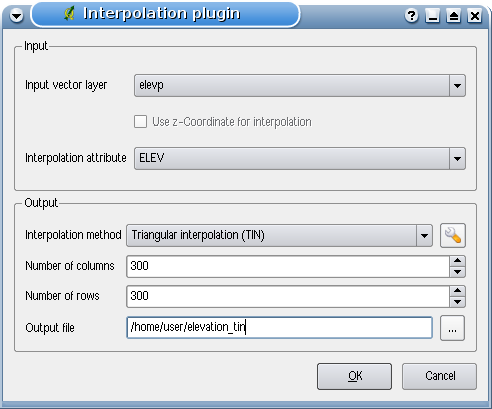
\includegraphics[clip=true, width=8cm]{interpolate_dialog}
\end{center}  
\end{figure}

\minisec{Das Plugin anwenden}\label{interpolation_usage}

\begin{enumerate}
  \item Starten Sie QGIS und laden Sie die CVS Tabelle \filename{elevp.csv}
mit H�heninformationen aus dem QGIS Beispieldatensatz mit Hilfe des Plugins
'Getrennter Text' aus Kapitel~\ref{label_dltext}. 
  \item Laden Sie das Interpolationsplugin mit dem Plugin Manager (siehe
Kapitel~\ref{sec:load_core_plugin}) und klicken Sie auf das Icon
\toolbtntwo{interpolation}{Interpolation} in der Werkzeugleiste, um den
Dialog zu starten.
  \item W�hlen Sie den Layer \selectstring{elevp}{} als Eingabevektorlayer und
Spalte \filename{ELEV} als Interpolationsattribut.
  \item W�hlen Sie \selectstring{Unregelm��iges Dreiecksnetz (TIN)}{} als
Interpolationsmethode, definieren Sie als Spalten- und Zellenzahl 1000. Das 
entspricht in etwa einer Aufl�sung in X- und Y-Richtung von 5000 metern. 
Als Ausgabedatei geben Sie \filename{elevation\_tin} an.
  \item Klicken Sie \button{Ok}.
  \item Doppelklicken Sie auf die Ergebniskarte \filename{elevation\_tin} in
der Legende, um den Dialog \dialog{Rasterlayereigenschaften} zu �ffnen und
w�hlen Sie im Reiter \tab{Darstellung} die Farbabbildung
\selectstring{Pseudofarben}{}. Oder Sie definieren eine neue Farbtabelle, wie
in Kapitel~\ref{label_rasterprop} beschrieben.
\end{enumerate}

In Abbildung~\ref{fig:interpolation_idw} sehen das Ergebnis einer
TIN-Interpolation mit einer Pixelaufl�sung von 5 km und der Farbabbildung
Pseudofarben. Die Interpolation ben�tigt einige Zeit, obwohl die Daten nur
den n�rdlichen Teil von Alaska abdecken.

\begin{figure}[ht]
   \begin{center}
   \caption{Interpolation von H�henpunkten mit der TIN-Methode \nixcaption}\label{fig:interpolation_tin}\smallskip
   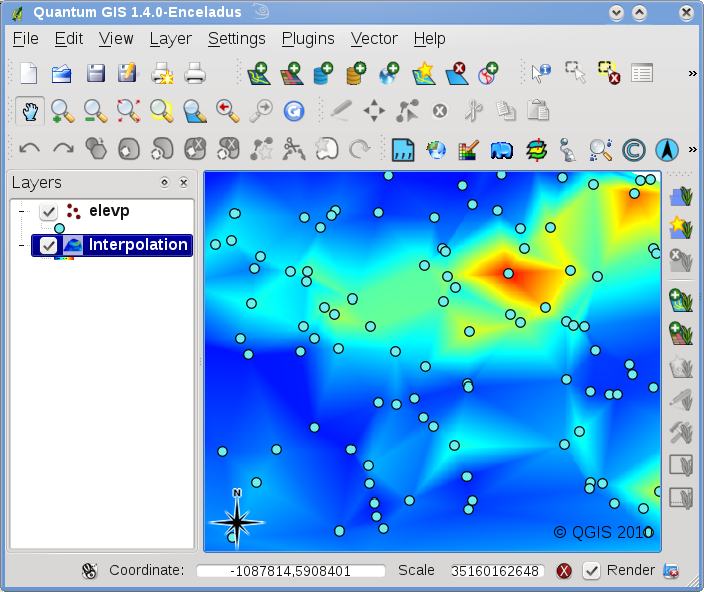
\includegraphics[clip=true, width=9cm]{interpolate_tin}
\end{center}  
\end{figure}

\newpage

